\documentclass{article}

\usepackage[utf8]{inputenc}
\usepackage[brazil]{babel}
\usepackage{amsmath, amssymb}
\usepackage{graphicx}
\usepackage{hyperref}
\usepackage{listings}
\usepackage{float}
\usepackage{xcolor}
\usepackage{pgffor}

\lstset{
    breaklines=true,
    breakatwhitespace=true,
    postbreak=\mbox{\textcolor{red}{$\hookrightarrow$}\space},
    basicstyle=\ttfamily\small,
    numbers=left,
    numberstyle=\tiny,
    stepnumber=1,
    numbersep=5pt,
    frame=single,
    showstringspaces=false,
    tabsize=4,
    language=Python
}

\title{Função de Correlação Cruzada e \textit{Pseudo-Random Binary Sequence}}
\author{Eduardo Henrique Basilio de Carvalho}
\date{\today}

\begin{document}

\maketitle

\section*{Questão 1}
Seja

\begin{equation}
    u[k] = 0.9\nu[k-1] + 0.8\nu[k-2] + 0.7\nu[k-3] + \nu[k]\label{eq:fir}
\end{equation}

onde $\nu[k]$ é ruído branco gaussiano com média zero e variância unitária.

\subsection*{a}

As funções de autocorrelação para $\nu$ e $u$ são apresentadas na Figura \ref{fig:fac_fir}.

\begin{figure}[H]
    \centering
    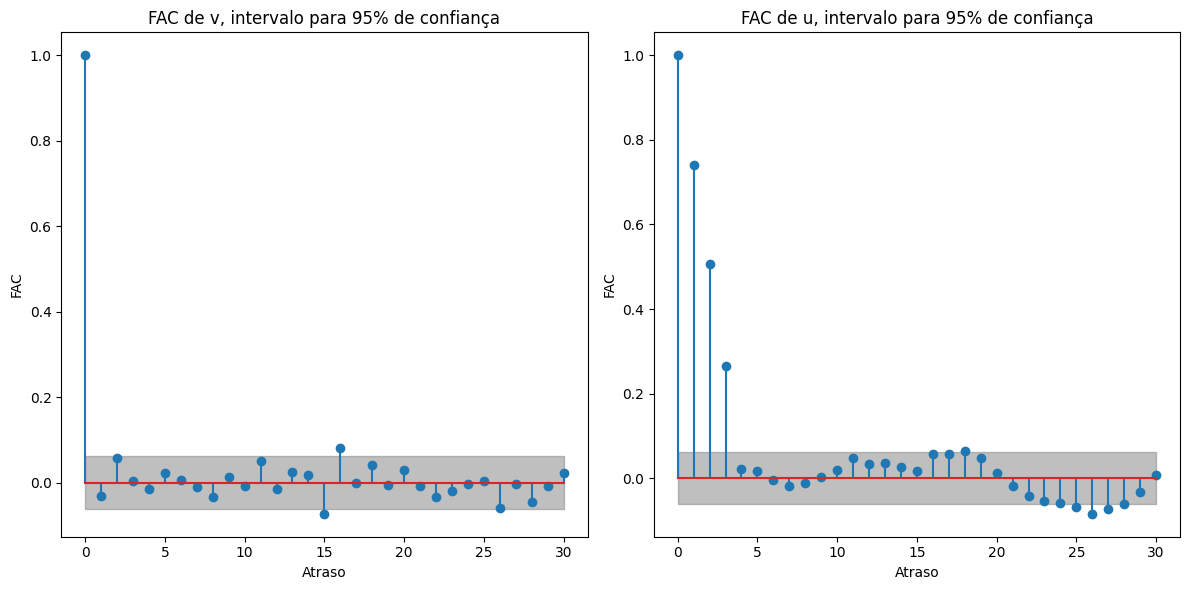
\includegraphics[width=\textwidth]{imagens/fac_fir.png}
    \caption{Função de autocorrelação para $\nu$ e $u$}
    \label{fig:fac_fir}
\end{figure}

Nesta, a FAC de $\nu$ condiz com o esperado, valor estatisticamente significante somente para $\tau = 0$. Esta curva é característica de sinais brancos, para os quais $\nu[k]$ não é função de $\nu[k-1]$. Para $u$, a FAC também é coerente com a expressão matemática. Apesar de $u[k]$ não ser função de $u[k-1]$, dois de seus três termos tomam valores comuns de $\nu$:

\begin{align*}
u[k-1] = &0.9v[k-2] + 0.8v[k-3] + 0.7[k-4] + v[k-1] \\
u[k] = 0.9v[k-1] + &0.8v[k-2] + 0.7v[k-3] + v[k]
\end{align*}

Assim, mesmo que $u[k]$ não seja efeito de $u[k-1]$, estes compartilham parte da causa, o que explica o decaimento suave da função de autocorrelação.

\subsection*{b}

A função de correlação cruzada entre $u$ e $\nu$ é apresentada na Figura \ref{fig:fcc_fir}.

\begin{figure}[H]
    \centering
    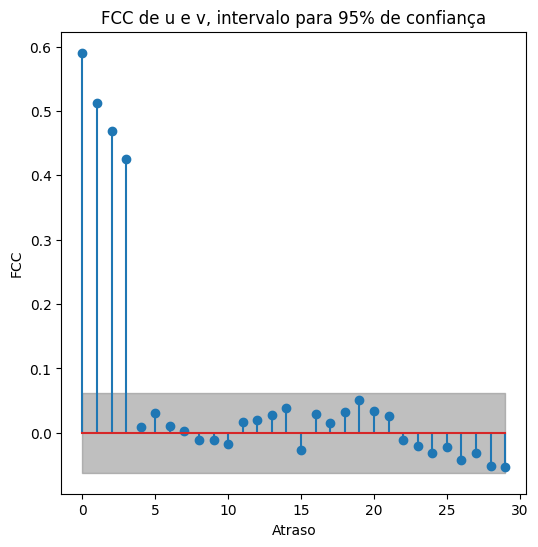
\includegraphics[width=\textwidth]{imagens/fcc_fir.png}
    \caption{Função de correlação cruzada entre $u$ e $\nu$}
    \label{fig:fcc_fir}
\end{figure}

Já neste caso, a correlação alta para os primeiros atrasos se dá pelo fato de $u$ ser função direta de $\nu$. Novamente, o decaimento suavizado nos primeiros valores decorre do comportamento passa baixas do sinal, definido por três valores consecutivos de $\nu$. É interessante notar que a queda repentina na correlação para $\tau = 4$ é coerente com a definição do sinal: como não há recursividade, não é esperada correlação entre $u[k]$ e $\nu[k-4]$.

\section*{Questão 2}
Seja

\begin{equation}
    H(z) = \frac{z + 0.5}{z^2 - 1.5z + 0.7}\label{eq:sis_2ordem}
\end{equation}

\subsection*{a, b, c}

As correlações cruzadas em ambos os sentidos são apresentadas na Figura \ref{fig:entrada_saida_fcc}.

\begin{figure}[H]
    \centering
    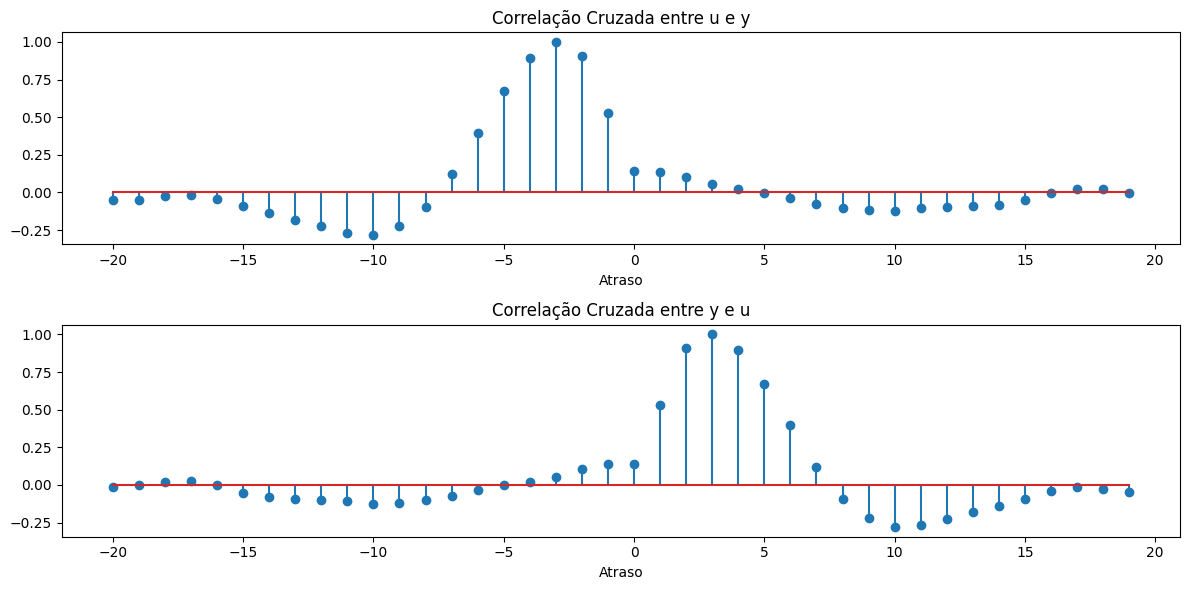
\includegraphics[width=\textwidth]{imagens/entrada_saida_fcc.png}
    \caption{Função de correlação cruzada entre (acima) entrada e saída e (abaixo) saída e entrada}
    \label{fig:entrada_saida_fcc}
\end{figure}

As curvas traçadas indicam que, quando a ordem dos parâmetros na chamada da função é \texttt{saída, entrada}, a correlação é mais significativa para atrasos positivos.

\subsection*{d}

A Figura \ref{fig:boxjenk_tempo} mostra as sequências carregadas do arquivo fornecido.

\begin{figure}[H]
    \centering
    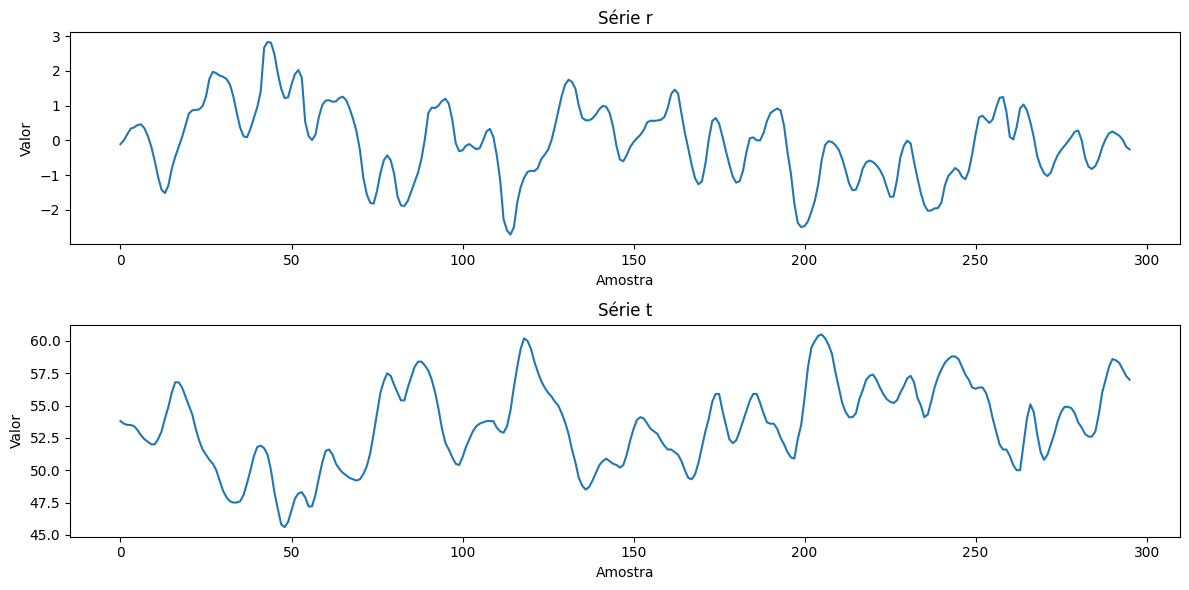
\includegraphics[width=\textwidth]{imagens/boxjenk_tempo.png}
    \caption{Sequências de entrada e saída do sistema Box-Jenkins}
    \label{fig:boxjenk_tempo}
\end{figure}

As funções de correlação cruzada entre \texttt{r} e \texttt{t} e entre \texttt{t} e \texttt{r} são apresentadas nas figuras \ref{fig:fcc_rt} e \ref{fig:fcc_tr}, respectivamente.

\begin{figure}[H]
    \centering
    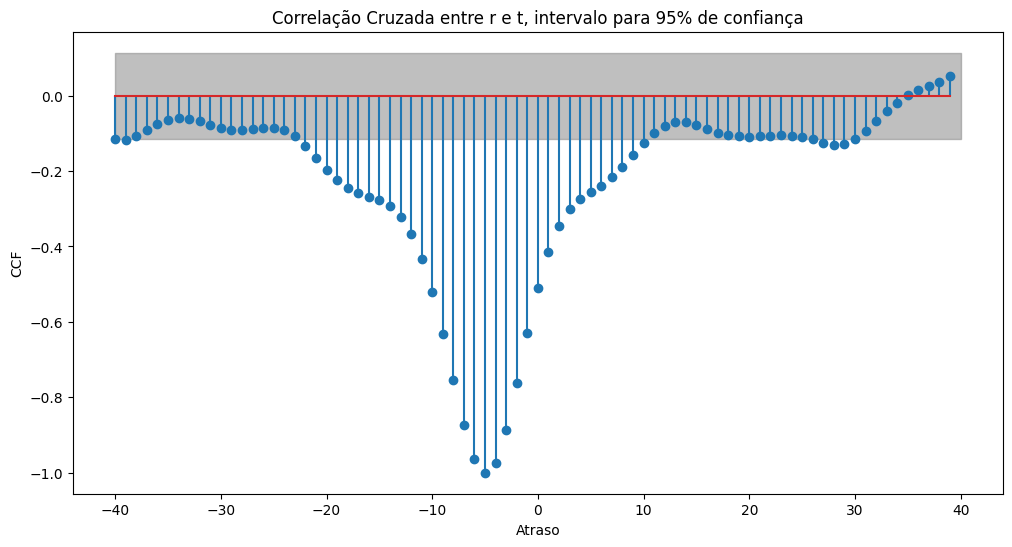
\includegraphics[width=\textwidth]{imagens/fcc_rt.png}
    \caption{Função de correlação cruzada entre \texttt{r} e \texttt{t}}
    \label{fig:fcc_rt}
\end{figure}

\begin{figure}[H]
    \centering
    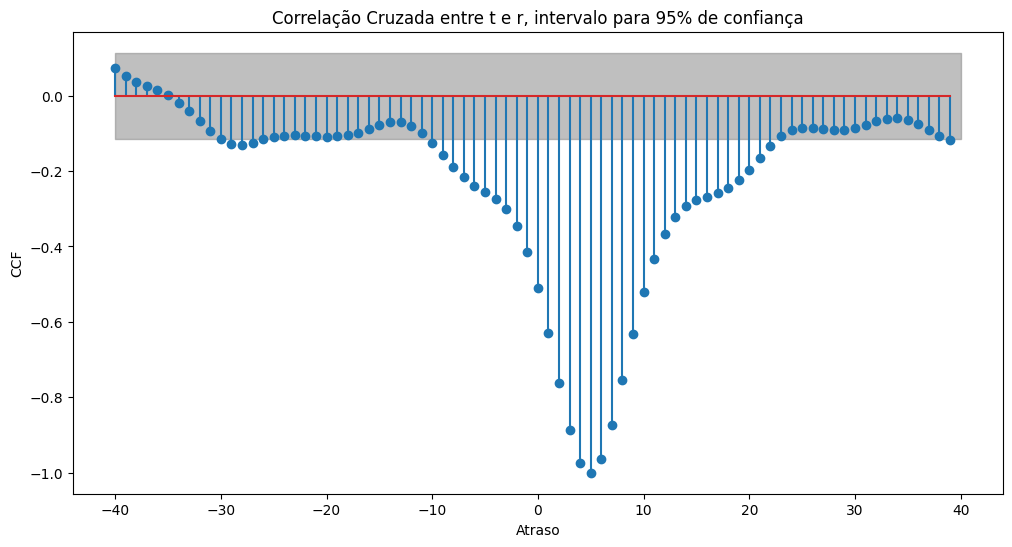
\includegraphics[width=\textwidth]{imagens/fcc_tr.png}
    \caption{Função de correlação cruzada entre \texttt{t} e \texttt{r}}
    \label{fig:fcc_tr}
\end{figure}

As curvas indicam que \texttt{t} e \texttt{r} são, respectivamente, saída e entrada.

\section*{Questão 3}

Para estimar a resposta ao impulso do sistema em \ref{eq:sis_2ordem}, a equação de Winer-Hopf foi utilizada. $u$, a entrada, é um sinal branco uniforme com média zero e amplitude 1. Sobre a saída, foi aplicado um ruído branco gaussiano com média 0 e desvio padrão $\sigma_\text{ruído} = 0.1\sigma_\text{y}$. A matriz $Ru$ foi construída conforme a definição de Toeplitz, com 40 linhas e colunas. O sistema construído foi resolvido com regularização de Tikhonov, com $\lambda = 0.01ru[0]$. A resposta ao impulso estimada é comparada com a referência na Figura \ref{fig:h_est_vs_ref}.

\begin{figure}[H]
    \centering
    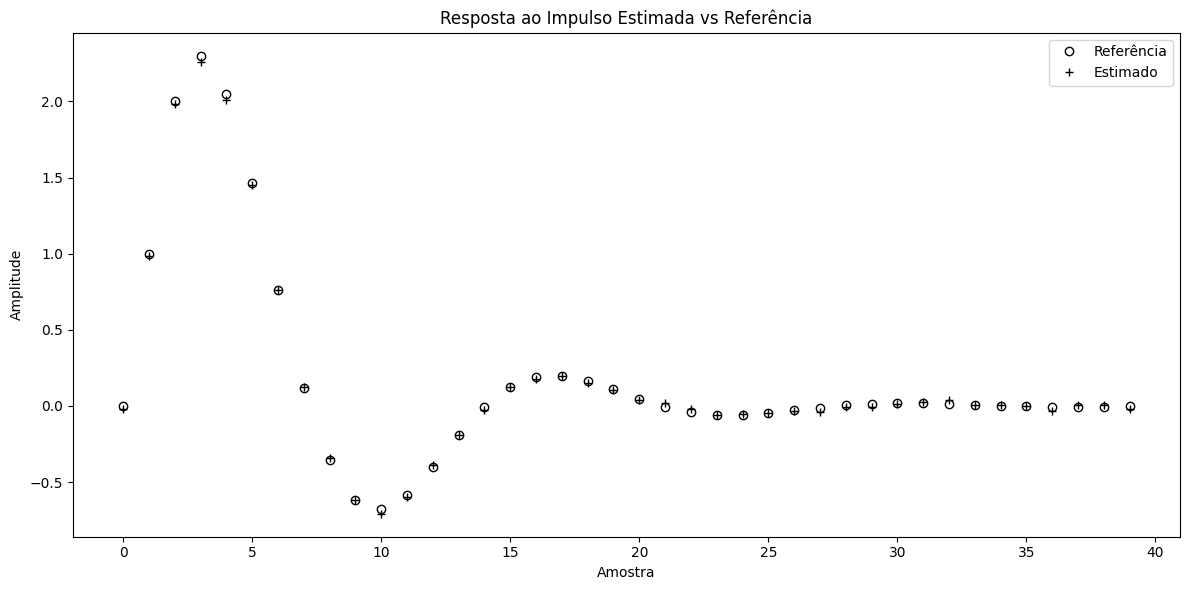
\includegraphics[width=\textwidth]{imagens/h_est_vs_ref.png}
    \caption{Resposta ao impulso estimada e de referência}
    \label{fig:h_est_vs_ref}
\end{figure}

\section*{Questão 4}

A figura \ref{fig:prbs_test} mostra os valores carregados do arquivo fornecido. Neste, é possível identificar a entrada como uma sequência pseudoaleatória binária e a saída como a resposta de um sistema dinâmico a esta entrada.

\begin{figure}[H]
    \centering
    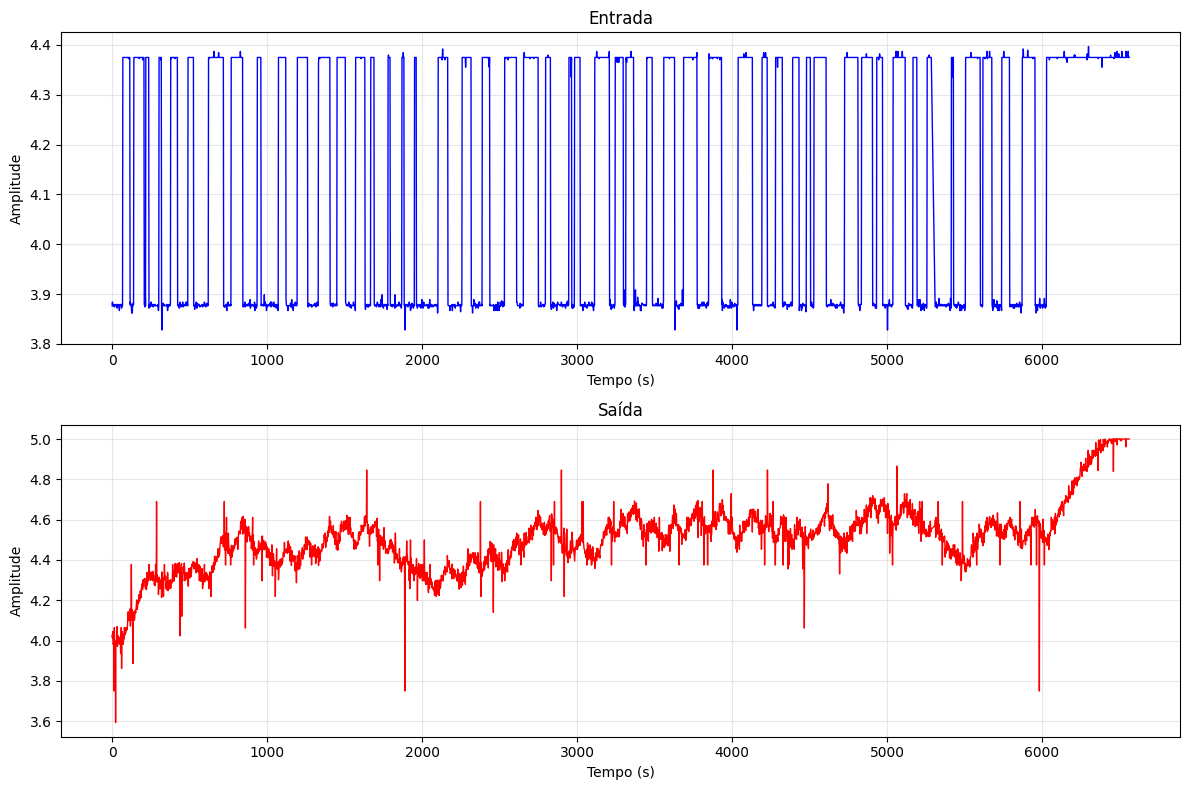
\includegraphics[width=\textwidth]{imagens/prbs_test.png}
    \caption{Sequências de entrada e saída do sistema}
    \label{fig:prbs_test}
\end{figure}

A função de autocorrelação da entrada é apresentada na Figura \ref{fig:prbs_fac}. Seu perfil condiz com o esperado para uma sequência PRBS, com correlação máxima para $\tau = 0$ e decaimento suave para os primeiros atrasos, decorrente da aleatoriedade limitada da sequência.

\begin{figure}[H]
    \centering
    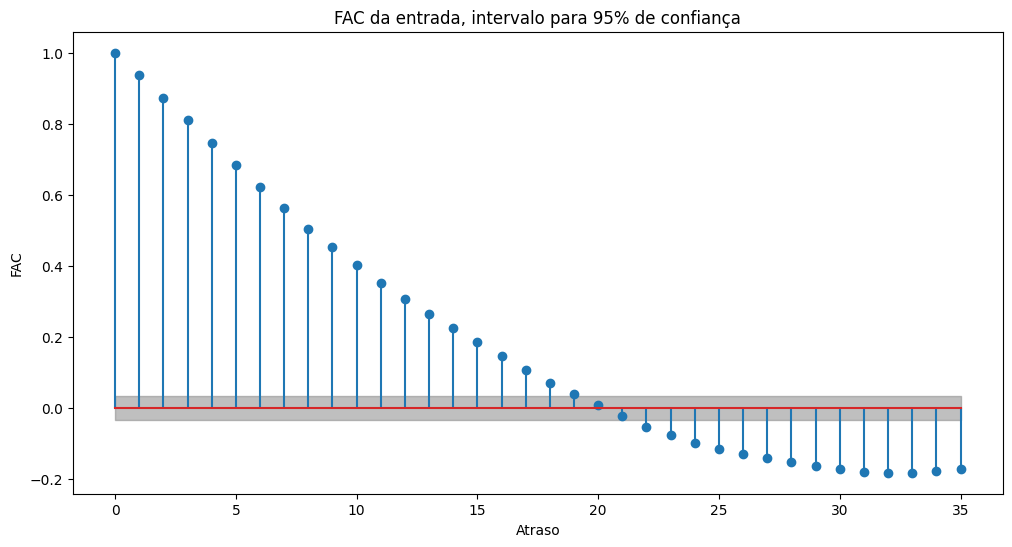
\includegraphics[width=\textwidth]{imagens/prbs_fac.png}
    \caption{Função de autocorrelação da entrada}
    \label{fig:prbs_fac}
\end{figure}

A resposta do sistema foi dividida em duas janelas, \texttt{[1000, 3000]} e \texttt{[3000, 5000]}, a fim de descartar os trechos iniciais e finais. A função de autocorrelação para ambas as janelas é apresentada na Figura \ref{fig:fac_saidas_prbs}.

\begin{figure}[H]
    \centering
    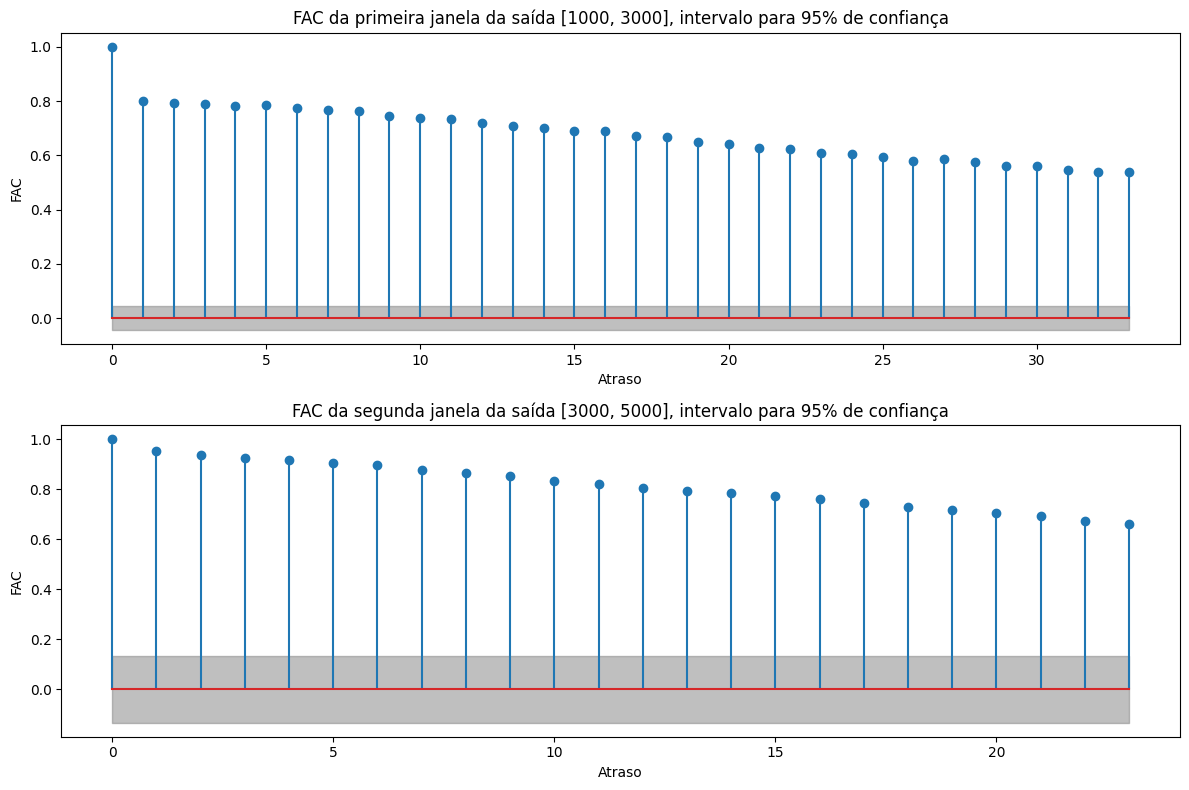
\includegraphics[width=\textwidth]{imagens/fac_saidas_prbs.png}
    \caption{Função de autocorrelação para as janelas \texttt{[1000, 3000]} (acima) e \texttt{[3000, 5000]} (abaixo)}
    \label{fig:fac_saidas_prbs}
\end{figure}

A primeira janela apresenta uma FAC com valor significativamente maior para $\tau = 0$ e queda repentina, o que pode indicar variação rápida do sistema. Já a segunda janela apresenta uma FAC com decaimento mais suave, o que pode indicar que o sistema está se aproximando de um regime permanente.

\section*{Questão 5}

Os pares de entrada e saída para diferentes \texttt{Tb} são apresentados nas figuras

\foreach \n in {1, 10, 100, 1000, 10000} {
     \ref{fig:prbs_\n.png}
}.

\foreach \n in {1, 10, 100, 1000, 10000} {
    \begin{figure}[H]
        \centering
        \includegraphics[width=\textwidth]{imagens/prbs_\n.png}
        \caption{Sequências de entrada e saída do sistema para $\text{Tb} = \n$}
        \label{fig:prbs_\n.png}
    \end{figure}
}

1000 amostras por bit parece produzir o sinal mais adequado para a identificação do sistema, já que décadas menores omitem a dinâmica do sistema, se asemelhando a ruído, e a década maior leva a muitos trechos em regime permanente. Tal resultado é aproximado da observação de que a faixa $\frac{\tau}{10} < Tb < \frac{\tau}{3}$ tende a ser adequada para a identificação de sistemas.

\end{document}
